\section{Methods}

\subsection{Data and task}

We use the Suturing task of the official JIGSAWS release. The metadata file lists \NTrials{} trials from eight surgeons (users B to I). Each user performed five trials, except user H, whose trial H002 has no label or fold entry in the official release and is therefore absent. The target is the self-reported skill level, novice (N, under 10 hours of robotic practice), intermediate (I, 10 to 100 hours) or expert (E, over 100 hours). Users B, G, H and I are novices (19 trials), C and F intermediates (10 trials), and D and E experts (10 trials). Each trial provides 76 kinematic channels sampled at 30\,Hz, namely the Cartesian position, rotation matrix, linear velocity, angular velocity and gripper angle of the two surgeon-side master manipulators and the two patient-side instruments, and two endoscope videos at 640$\times$480 pixels and 30 frames per second. We use the patient-side instruments for the kinematic features, because they are the tools that act on the tissue and the master signals largely duplicate them under teleoperation, and we use the left camera view (capture1) for the video features. Trials last between \DurMin{} and \DurMax{}\,s (median \DurMedian{}\,s), and novices are slower on average (Figure~\ref{fig:data}). Neither the gesture transcriptions nor the OSATS scores are used by any model.

\begin{figure}[htbp]
\centering
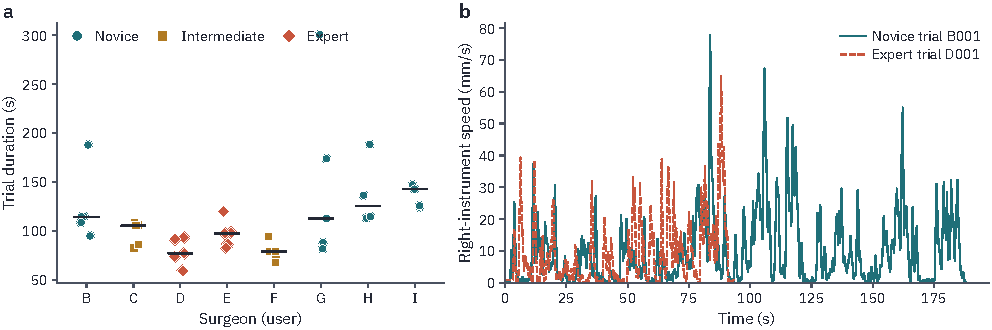
\includegraphics{fig2_data.pdf}
\caption{(a) Trial duration per surgeon, coloured by skill level; bars mark the median. (b) Speed of the right patient-side instrument, smoothed over 0.5\,s, in a novice trial (B001) and an expert trial (D001). The expert finishes in about half the time with a comparable peak speed.}
\label{fig:data}
\end{figure}

\subsection{Workflow}

Figure~\ref{fig:pipeline} summarises the pipeline. Each trial is turned into fixed-length feature vectors, one per feature block. A block is classified by a standardised, L2-regularised logistic regression whose regularisation strength is chosen inside the training surgeons. Multimodal models either concatenate blocks before classification (early fusion) or average the class probabilities of a kinematic and a video classifier (late fusion). Everything is evaluated with the eight official LOUO folds of the JIGSAWS skill-detection setup.

\begin{figure}[htbp]
\centering
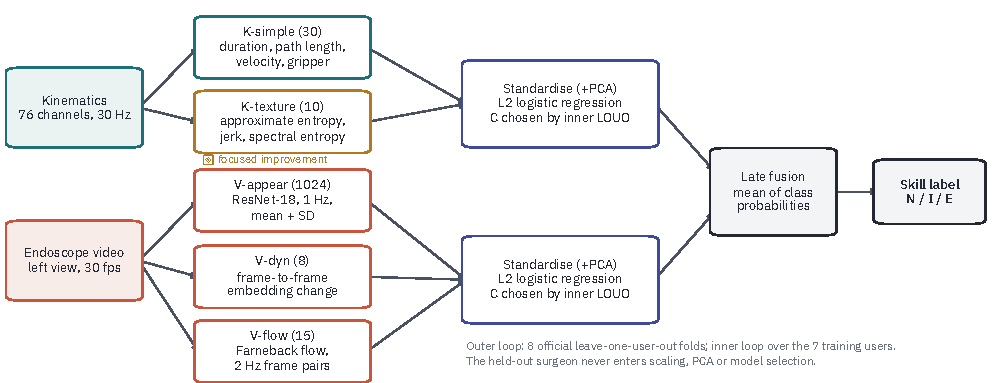
\includegraphics{fig1_pipeline.pdf}
\caption{Workflow. Kinematic and video feature blocks are extracted per trial and classified by regularised logistic regression; late fusion averages the class probabilities of one kinematic and one video classifier. The K-texture block is the focused improvement. Numbers in brackets are feature dimensions. All fitting, including scaling, PCA and the choice of the regularisation strength, uses only the training surgeons of each fold.}
\label{fig:pipeline}
\end{figure}

\subsection{Kinematic features}

The kinematics-only baseline (K-simple, 30 features) implements the statistics named in the task specification. For each patient-side instrument we compute the path length as the summed distance between consecutive tool-tip positions; the mean, standard deviation and 90th percentile of the linear speed; the mean and standard deviation of the angular speed; the idle fraction, defined as the share of samples with linear speed below 5\,mm/s; the economy of motion, defined as path length divided by the diagonal of the bounding box of the tool-tip trajectory; and five gripper statistics, namely the mean, standard deviation and range of the gripper angle, its total absolute change and the number of opening-and-closing cycles, counted as upward crossings of the mean of a 0.5\,s moving average. Four trial-level features complete the block: the duration in seconds, the correlation between the speeds of the two instruments, the share of time in which both are idle, and the log ratio of the two path lengths. All are standard descriptors of efficiency and bimanual coordination \citep{reiley2011review, lefor2020motion}.

The motion-texture block (K-texture, 10 features) is the focused improvement and follows the background reference \citep{zia2018rmis}. For each instrument we compute approximate entropy \citep{pincus1991apen} of the linear speed, the angular speed and the gripper angle, each resampled to 10\,Hz, with embedding dimension $m = 2$ and tolerance $r = 0.2$ times the standard deviation of the signal; the log dimensionless jerk of the velocity profile \citep{hogan2009smoothness}; and the normalised spectral entropy of the speed. These features describe how regular and smooth a movement is rather than how fast or how long, which is the property that should separate a fluent expert from a hesitant novice even when both take a similar time.

\subsection{Video features}

Frames are decoded once per trial. Every 30th frame (1\,Hz, \NFramesOneHz{} frames in total) is resized to 224$\times$224 pixels and passed through an ImageNet-pretrained ResNet-18 \citep{he2016resnet} with the classification layer removed, giving a 512-dimensional embedding per frame. The appearance block (V-appear, 1024 features) is the mean and the standard deviation of these embeddings over the trial; because 1024 dimensions are far too many for 34 training trials, a PCA with 4, 8 or 16 components is fitted inside each training fold. The scene-dynamics block (V-dyn, 8 features) summarises how fast the view changes: from the cosine distance between consecutive 1\,Hz embeddings we take the mean, standard deviation, 10th, 50th and 90th percentiles and coefficient of variation, and from the Euclidean distance the mean and standard deviation. A constant appearance offset, such as the lighting or the layout of the practice board in a given session, cancels in these differences, so V-dyn should carry less information about the recording setup than V-appear while still reflecting instrument motion and tissue change. The optical-flow block (V-flow, 15 features) uses Farneback dense flow \citep{farneback2003flow} on pairs of consecutive frames sampled at 2\,Hz (\NPairsTwoHz{} pairs) and downscaled to 320$\times$240 pixels. For each pair we compute the mean, standard deviation and 90th percentile of the flow magnitude, the fraction of pixels moving faster than 0.5 pixels per frame, and the magnitude-weighted entropy of the flow direction over eight bins, and we summarise each of these five series over the trial by its mean, standard deviation and 90th percentile.

\subsection{Classifiers and fusion}

Every block is classified by the same model: standardisation, optional PCA (V-appear only), a second standardisation after PCA, and multinomial logistic regression with an L2 penalty, balanced class weights and the L-BFGS solver \citep{pedregosa2011sklearn}. The inverse regularisation strength $C$ is chosen from $\{0.01, 0.03, 0.1, 0.3, 1, 3, 10\}$ and, for V-appear, the number of components from $\{4, 8, 16\}$. Late fusion averages the class probabilities of the kinematic classifier and one video classifier with equal weights; equal weighting was chosen because 34 training trials are too few to estimate a fusion weight reliably. Early fusion concatenates K-simple with V-dyn and fits one classifier. The primary multimodal model, fixed before any result was seen, is the late fusion of K-simple and V-dyn (M3). V-dyn was chosen as the primary video block for the first-principles reason given above and because an earlier exploratory analysis by our group on the same 39 trials had found embedding-change statistics to be the most promising video descriptor. Since that earlier analysis looked at out-of-fold results on the same data, the choice is not free of selection, and we therefore report all three video blocks and all four fusion variants.

\subsection{Evaluation protocol}

We use the official JIGSAWS folds in \texttt{Suturing/unBalanced/SkillDetection/UserOut}; the code checks that each fold holds out exactly one surgeon, which gives eight folds with 34 or 35 training trials. Hyperparameters are selected by an inner LOUO loop over the seven training surgeons of each outer fold, maximising the inner pooled macro-F1, with ties resolved towards stronger regularisation. When the outer fold holds out an intermediate or expert surgeon, only one surgeon of that class remains, and the inner fold that would hold it out has no training example of the class; such inner folds are skipped (one per affected outer fold). The held-out surgeon therefore never influences standardisation, PCA, feature residualisation or model selection.

The primary metric is macro-F1 computed once over the 39 pooled out-of-fold predictions. Because the label is constant within a surgeon, each LOUO test fold contains a single class and per-fold macro-F1 is undefined for the two absent classes, so pooling is the only well-defined form of the metric. We also report accuracy, per-class F1, the confusion matrix and accuracy per surgeon. With eight surgeons the uncertainty is large, so we quantify it in two ways that respect the grouping of trials. A user-level bootstrap resamples the eight surgeons with replacement 2000 times and gives percentile intervals for macro-F1 and for paired differences between models. An exact permutation test reassigns the skill labels among the surgeons while keeping each surgeon's trials together; with four novice, two intermediate and two expert surgeons there are $8!/(4!\,2!\,2!) = 420$ distinct assignments, so the null distribution of macro-F1 for fixed predictions is enumerated exactly and the smallest attainable $p$-value is $1/420$. Three comparisons were declared in advance: kinematics against the majority class (M1 vs M0), adding video to kinematics (M3 vs M1) and adding motion texture (M4 vs M1). A difference is called supported only if its bootstrap interval excludes zero. The complete protocol, including the model list in Table~\ref{tab:main}, was written to \texttt{PROTOCOL.md} before the pipeline was run, and every model was evaluated exactly once.

\subsection{Shortcut audit}

Two kinds of shortcut are plausible here. A feature block can identify the surgeon, in which case a classifier can reproduce training labels by recognising people, and that ability does not transfer to an unseen surgeon. We measure this with an identity probe: an eight-way surgeon classifier on each block, evaluated with stratified five-fold cross-validation over trials, whose balanced accuracy is compared with the chance level of 1/8. The second shortcut is pace. Novices are slower on average, so a model may rank trials by duration and call the result skill. We test this with a duration-only classifier (C1) and with K-simple after every feature has been residualised on log duration (C2, and C2t for the block with texture), with the regression fitted on the training surgeons only.

\subsection{Differences from existing work}
\label{sec:differences}

Our approach differs from the background reference and most related work in four ways. First, the reported numbers come from a protocol fixed before the run: every model, metric and comparison was written down in advance and each model was evaluated once, so the choice of the reported model could not depend on the test results. Second, we treat the eight surgeons rather than the 39 trials as the unit of uncertainty, reporting user-level bootstrap intervals and an exact permutation test over all 420 label assignments instead of a single accuracy, and we report macro-F1 so that the two small classes count as much as the novices. Third, we measure two shortcuts directly, the surgeon identity carried by each feature block and the share of the decision explained by trial duration, instead of assuming that a high score reflects skill. Fourth, the scene-dynamics descriptor V-dyn is designed to cancel the static appearance of a recording session, which whole-frame appearance features retain, and we test directly whether this reduces the identity shortcut.

\subsection{External resources and our contribution}

We used the JIGSAWS data and its official split files, the ImageNet weights of ResNet-18 distributed with torchvision \citep{paszke2019pytorch}, the Farneback implementation of OpenCV \citep{bradski2000opencv}, and scikit-learn \citep{pedregosa2011sklearn}, NumPy \citep{harris2020numpy} and SciPy \citep{virtanen2020scipy} for the classifiers and signal processing. No released skill-assessment code was used. The group implemented the data loading and fold checks, all feature definitions, the nested LOUO evaluation, the fusion models, the bootstrap and exact permutation analyses, the shortcut audit and all figures.
